\section{mr::sampler3D Struct Reference}
\label{structmr_1_1sampler3D}\index{mr::sampler3D@{mr::sampler3D}}
{\tt \#include $<$mr\-Sampler.h$>$}

Inheritance diagram for mr::sampler3D::\begin{figure}[H]
\begin{center}
\leavevmode
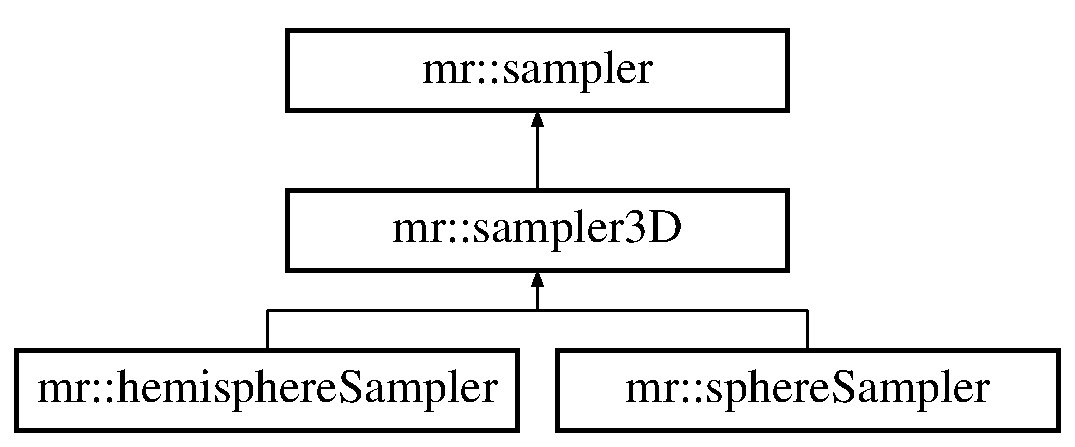
\includegraphics[height=3cm]{structmr_1_1sampler3D}
\end{center}
\end{figure}
\subsection*{Public Member Functions}
\begin{CompactItemize}
\item 
{\bf sampler3D} ()
\begin{CompactList}\small\item\em Constructor for adaptive sampling. \item\end{CompactList}\item 
{\bf sampler3D} (const mi\-Uint \&num\-Samples)
\begin{CompactList}\small\item\em Constructor for fixed sampling. num\-Samples HAS to be mi\-Uint\&. \item\end{CompactList}\item 
{\bf $\sim$sampler3D} ()
\item 
mi\-Vector \& {\bf direction} ()
\begin{CompactList}\small\item\em Return direction for this sample. \item\end{CompactList}\end{CompactItemize}
\subsection*{Public Attributes}
\begin{CompactItemize}
\item 
double {\bf samples} [2]
\begin{CompactList}\small\item\em mi\_\-sample() auxiliaries to store 2 random numbers \item\end{CompactList}\item 
mi\-Vector {\bf dir}
\begin{CompactList}\small\item\em Final sampling direction for this sample. \item\end{CompactList}\end{CompactItemize}


\subsection{Constructor \& Destructor Documentation}
\index{mr::sampler3D@{mr::sampler3D}!sampler3D@{sampler3D}}
\index{sampler3D@{sampler3D}!mr::sampler3D@{mr::sampler3D}}
\subsubsection{\setlength{\rightskip}{0pt plus 5cm}mr::sampler3D::sampler3D ()\hspace{0.3cm}{\tt  [inline]}}\label{structmr_1_1sampler3D_a0}


Constructor for adaptive sampling. 

\index{mr::sampler3D@{mr::sampler3D}!sampler3D@{sampler3D}}
\index{sampler3D@{sampler3D}!mr::sampler3D@{mr::sampler3D}}
\subsubsection{\setlength{\rightskip}{0pt plus 5cm}mr::sampler3D::sampler3D (const mi\-Uint \& {\em num\-Samples})\hspace{0.3cm}{\tt  [inline]}}\label{structmr_1_1sampler3D_a1}


Constructor for fixed sampling. num\-Samples HAS to be mi\-Uint\&. 

\index{mr::sampler3D@{mr::sampler3D}!~sampler3D@{$\sim$sampler3D}}
\index{~sampler3D@{$\sim$sampler3D}!mr::sampler3D@{mr::sampler3D}}
\subsubsection{\setlength{\rightskip}{0pt plus 5cm}mr::sampler3D::$\sim${\bf sampler3D} ()\hspace{0.3cm}{\tt  [inline]}}\label{structmr_1_1sampler3D_a2}




\subsection{Member Function Documentation}
\index{mr::sampler3D@{mr::sampler3D}!direction@{direction}}
\index{direction@{direction}!mr::sampler3D@{mr::sampler3D}}
\subsubsection{\setlength{\rightskip}{0pt plus 5cm}mi\-Vector\& mr::sampler3D::direction ()\hspace{0.3cm}{\tt  [inline]}}\label{structmr_1_1sampler3D_a3}


Return direction for this sample. 



\subsection{Member Data Documentation}
\index{mr::sampler3D@{mr::sampler3D}!dir@{dir}}
\index{dir@{dir}!mr::sampler3D@{mr::sampler3D}}
\subsubsection{\setlength{\rightskip}{0pt plus 5cm}mi\-Vector {\bf mr::sampler3D::dir}}\label{structmr_1_1sampler3D_o1}


Final sampling direction for this sample. 

\index{mr::sampler3D@{mr::sampler3D}!samples@{samples}}
\index{samples@{samples}!mr::sampler3D@{mr::sampler3D}}
\subsubsection{\setlength{\rightskip}{0pt plus 5cm}double {\bf mr::sampler3D::samples}[2]}\label{structmr_1_1sampler3D_o0}


mi\_\-sample() auxiliaries to store 2 random numbers 



The documentation for this struct was generated from the following file:\begin{CompactItemize}
\item 
{\bf mr\-Sampler.h}\end{CompactItemize}
